%!TEX root = ../aufgabenstellung.tex

\section{Entwurf \enquote{Ampel im Straßenverkehr} \points{25+15}}

In dieser Aufgabe wird eine Steuerungssoftware für Ampeln betrachtet, die in dem in Aufgabe 1 genannten Verkehrssystem eingesetzt werden soll.

\begin{center}
	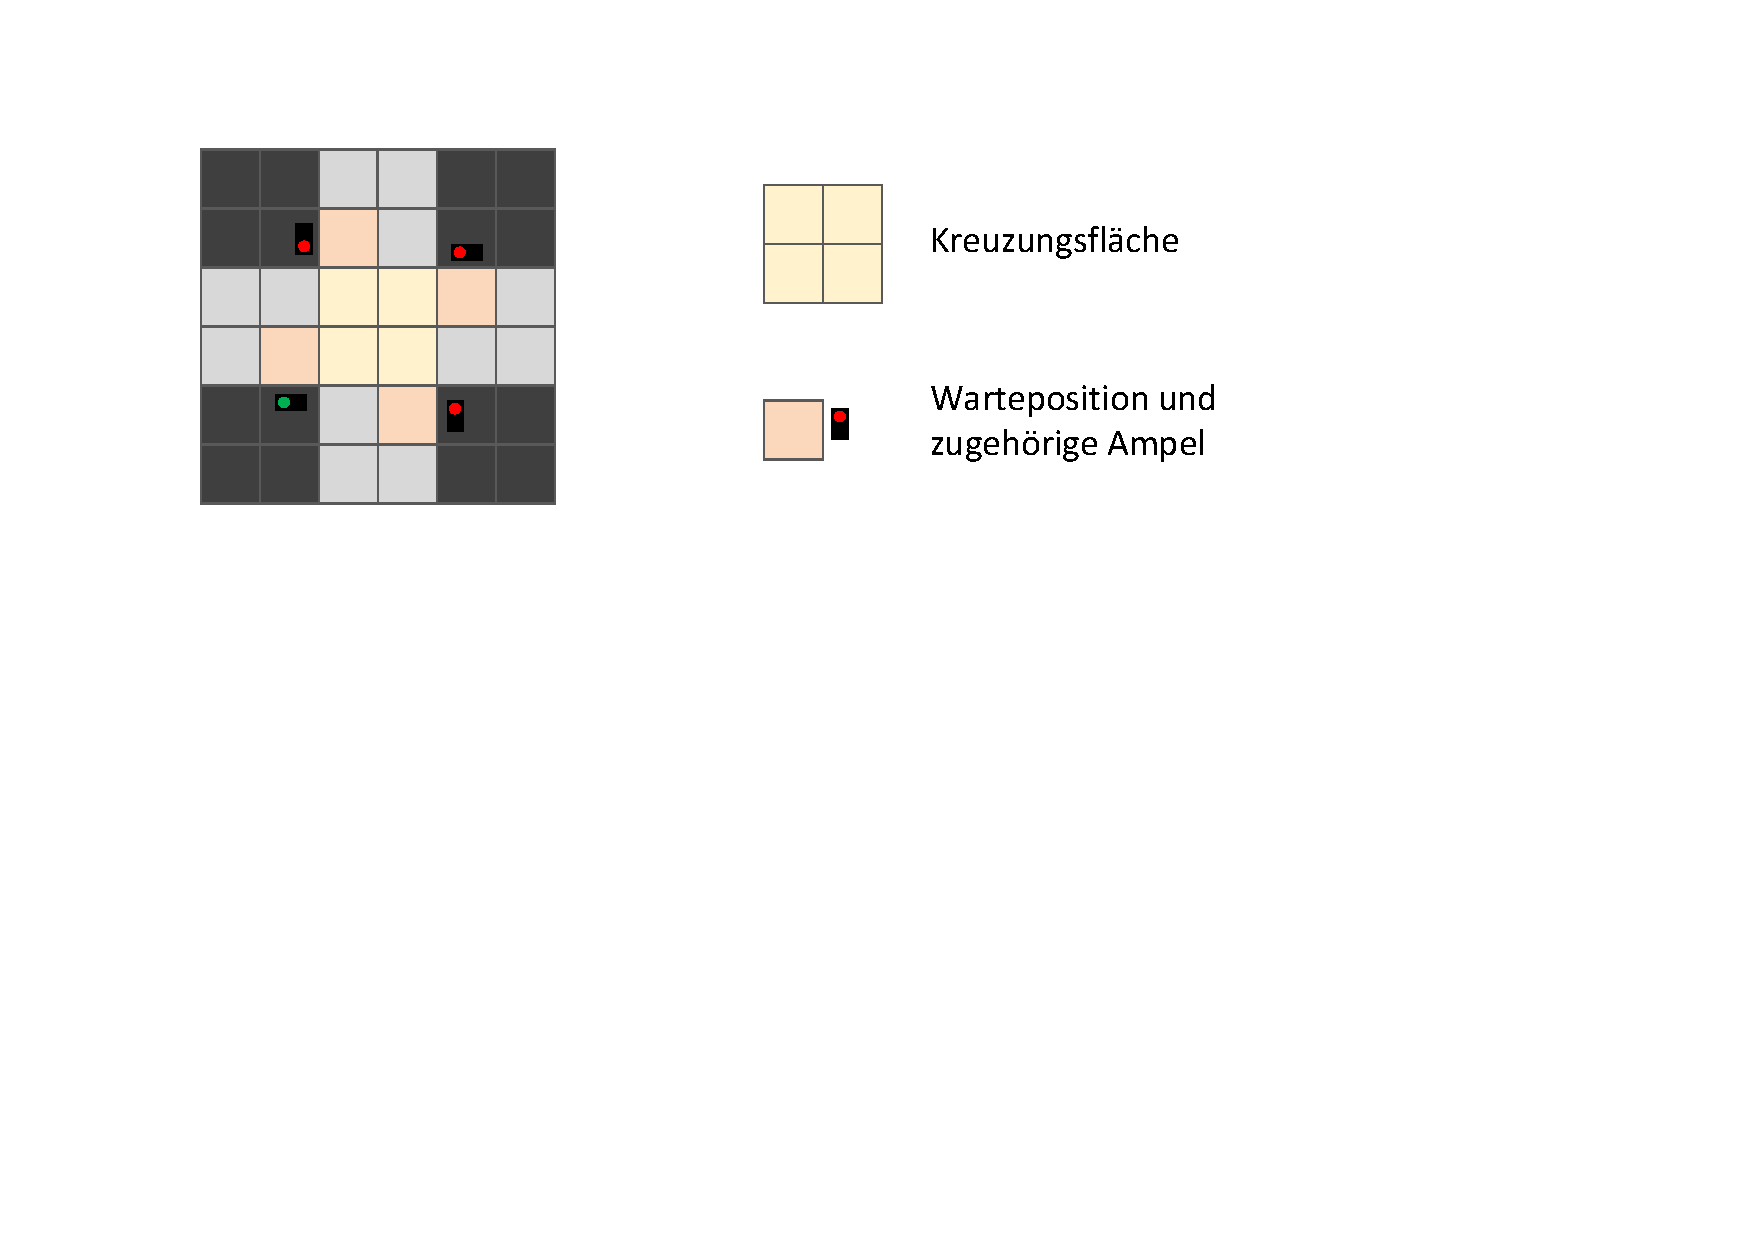
\includegraphics[width=0.6\textwidth]{verkehr_ampel_skizze.pdf}
\end{center}

Die Steuerungssoftware wird durch eine aktive Klasse \texttt{TrafficLightControl} umgesetzt.
Ein \texttt{TrafficLightControl}-Objekt ist immer für die Verkehrssteuerung auf einer kompletten Kreuzung zuständig.

Die Steuerung des Verkehrsflusses erfolgt durch das Wechseln der angezeigten Farbe bei den jeweils vier zugehörigen Ampeln, die in die Himmelsrichtungen Nord, Ost, Süd und West zeigen.
Für jede der Ampeln an einer Kreuzung steht dem \texttt{TrafficLightControl}-Objekt ein \texttt{Lamp}-Objekt zur Steuerung zur Verfügung.
Eine Ampel kann immer nur entweder rot oder grün anzeigen. 

Zusätzlich verfügt die Steuerungssoftware über fünf Sensoren, die feststellen können, ob sich in einem Bereich Roboter aufhalten oder nicht. Ein Sensor beobachtet die zentrale Fläche der Kreuzung, außerdem gibt es für jede Himmelsrichtung einen weiteren Sensor, der die Warteposition vor den Ampeln beobachtet. Jeder der Sensoren kann über ein \texttt{Sensor}-Objekt angesteuert werden.



\begin{enumerate}[a) ]
	\item Modellieren Sie ein Klassendiagramm für die Steuerungsoftware der Ampel.	Neben dem obenstehenden Text ist dazu die folgende beispielhafte Sequenz von Interaktionen vorgegeben:

	\begin{center}
		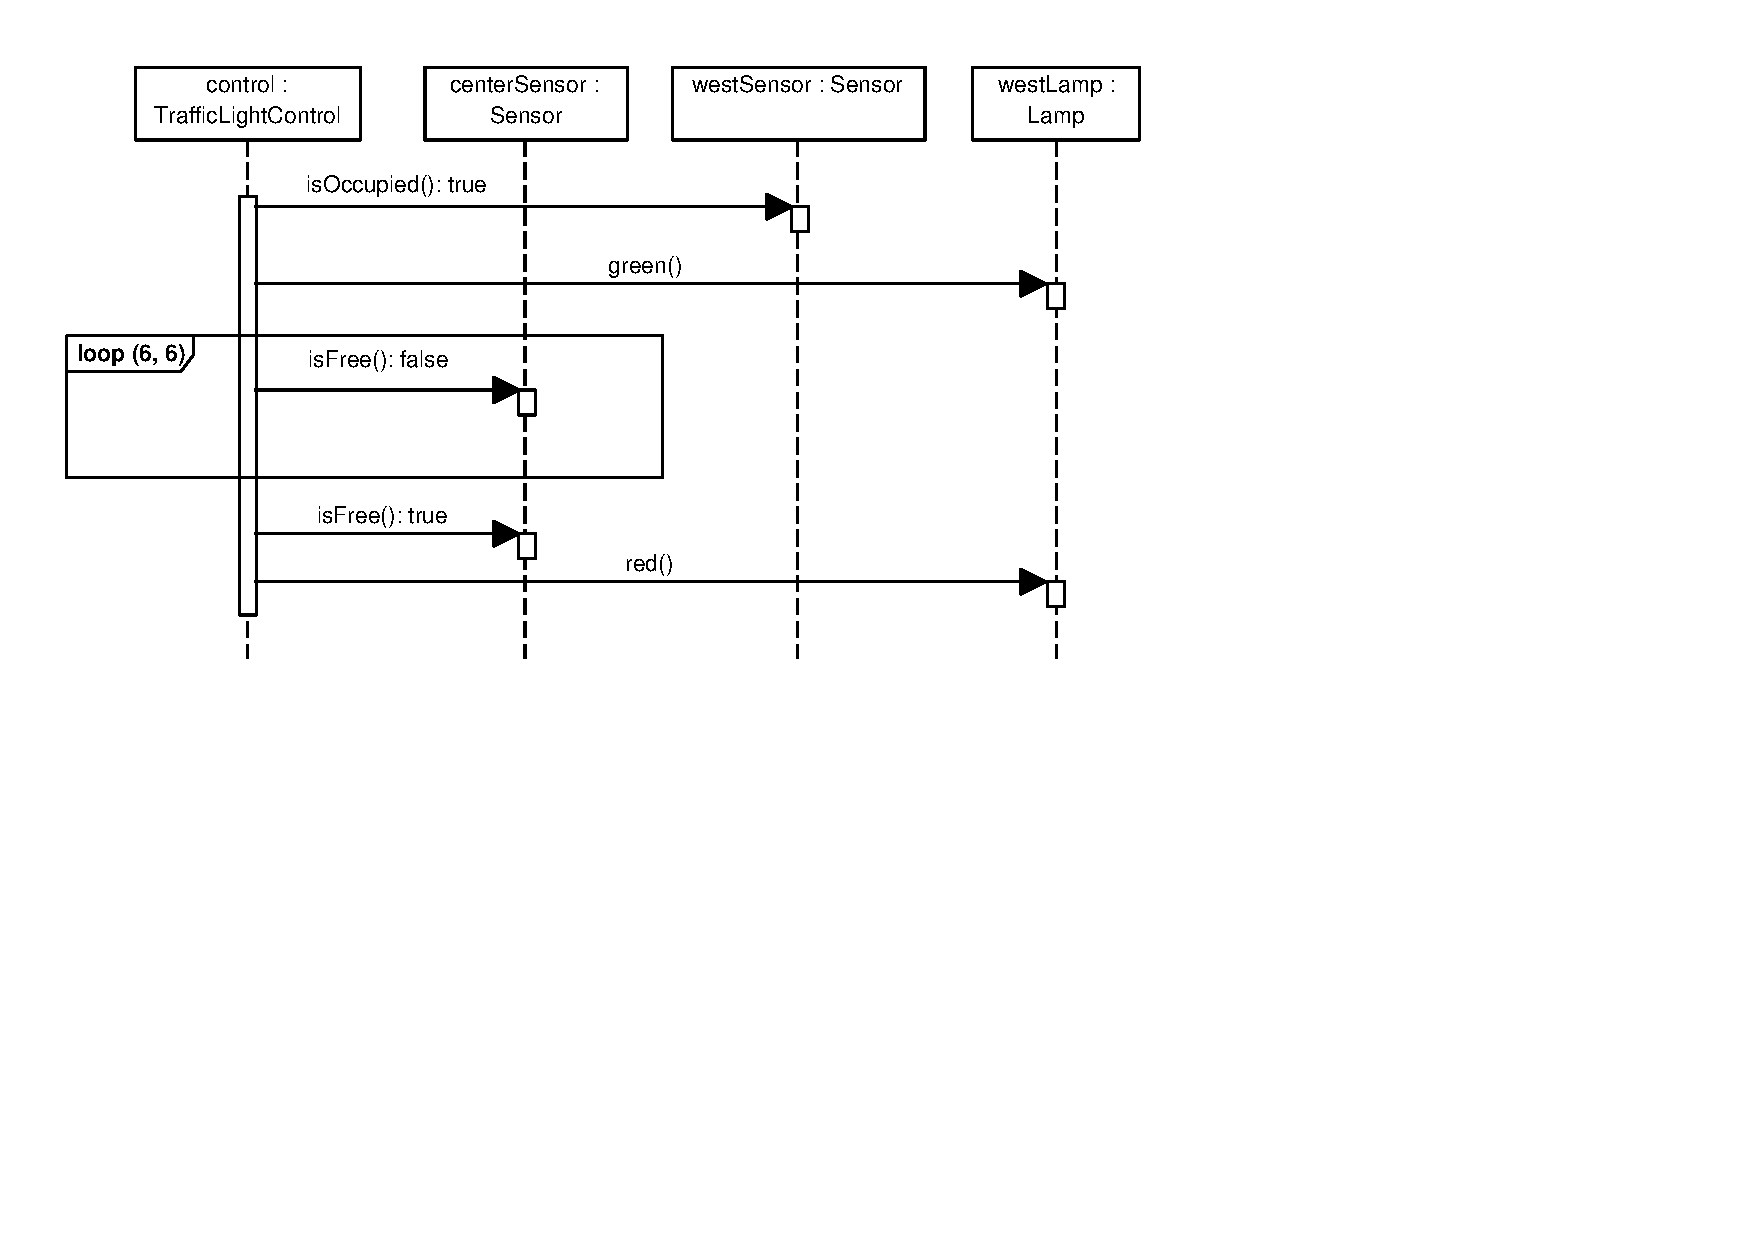
\includegraphics[width=0.6\textwidth]{verkehr_ampel_sequenzdiagramm.pdf}
	\end{center}

	Achten Sie auf Konsistenz zum Sequenzdiagramm. 
	Nehmen Sie an, dass die Bestandteile der Ampelsteuerung für alle vier Himmelsrichtungen äquivalent funktionieren und benannt sind, auch wenn nicht alle Richtungen im Sequenzdiagramm vorkommen. \points{7}
\end{enumerate}



\solutionbox{
	\red{Musterlösungen sind nicht öffentlich, können aber auf Anfrage bereitgestellt werden.}
}

\solution{\newpage}








\begin{enumerate}[a) ,resume]
	\item Modellieren Sie das Verhalten der aktiven Klasse \texttt{TrafficLightControl} mit einem UML-Zustands\-diagramm, sodass folgende Eigenschaften erfüllt werden:
	\begin{itemize}
		\item Die Ampeln in den einzelnen Himmelsrichtungen werden reihum einzeln auf grün geschaltet, die übrigen drei Ampeln sind währenddessen rot.
		\item Eine Ampel wird erst dann auf grün gestellt, wenn sich auf der Kreuzungsfläche keine Roboter mehr befinden. Im pessimistischsten Fall kann angenommen werden, dass eine Durchquerung einer Kreuzung für einen Roboter nicht länger als 3 Sekunden dauert.
		\item Zeiten, in denen alle vier Ampeln gleichzeitig rot zeigen, sollen möglichst kurz gehalten werden (zumindest sofern auf einer Warteposition noch ein Roboter wartet).
		\item Kein Roboter, der die Warteposition direkt vor der Ampel erreicht, soll auf dieser länger als 30 Sekunden warten müssen.
	\end{itemize}

	In Situationen, wo regelmäßig eine Abfrage erfolgen muss (z.B. bei Warten bis die Kreuzungsfläche frei ist), verwenden Sie \texttt{after 100ms} als Trigger und \underline{nicht} den Trigger \texttt{when}.

	Achten Sie bei der Modellierung auf Konsistenz zu Ihrem Klassendiagramm. 
	Der beispielhafte Ablauf im bei Teilaufgabe a) gegebenen Sequenzdiagramm muss \underline{nicht} beachtet werden. \points{18}
	
	\fbox{\parbox{0.95\textwidth}{
		\textbf{Hinweis:} Nutzen Sie für diese und die folgende Teilaufgabe die YAKINDU Statechart Tools für die Modellierung. Laden Sie bei der Abgabe neben der üblichen PDF-Datei ein \texttt{.zip}-Archiv im Moodle hoch, welches die \texttt{simpletraffic\_light.ysc}-Datei mit Ihren Diagramm enthält.
		\newline
		\newline
		Wir stellen Ihnen für diese Übung ein Framework zur Verfügung, mit dem Sie das durch ihr Zustandsdiagramm definierte Fahrverhalten der Roboter selbst erproben und beobachten können.
		Weitere Informationen zur Installation  und Verwendung der YAKINDU Statechart Tools und des Simulators finden Sie in dem im Moodle hinterlegten Dokument \texttt{\red{Toolhinweise.pdf}}. 
		\newline
		\newline
		Beachten Sie, dass die Diagramm-Syntax in den YAKINDU Statechart Tools von der üblichen UML-Syntax abweicht. Die wichtigsten Besonderheiten sind ebenfalls in \texttt{\red{Toolhinweise.pdf}} kurz aufgelistet. Für die Klausur müssen Sie nur die Syntax von UML-Zustandsdiagrammen beherrschen.
	}}
\end{enumerate}


\solutionbox{
	\red{Musterlösungen sind nicht öffentlich, können aber auf Anfrage bereitgestellt werden.}
}

\solution{\newpage}







\begin{enumerate}[a) ,resume]
	\item \textbf{Bonusaufgabe:} Verbessern Sie Ihre Lösung aus Teilaufgabe b), sodass der Roboterverkehr insgesamt effizienter wird (und die Roboter im Durchschnitt schneller ihre Ziele erreichen). Mögliche Ansätze dafür:
	\begin{itemize}
		\item Eine Ampel schaltet in einer Himmelsrichtung nur dann auf grün, wenn bereits ein Roboter auf der Warteposition steht.
		\item Ampelphasen werden verkürzt falls keine Roboter auf die Warteposition nachrücken.
		\item Es wird beachtet, in welche Richtung die Roboter abbiegen wollen, um ggf. mehrere Ampeln gleichzeitig auf grün schalten zu können.
		Dazu kann angenommen werden, dass die  \texttt{Sensor}-Objekte die zusätzliche Methode \texttt{getDirection()} zur Verfügung stellt, die \texttt{Direction.LEFT} oder \texttt{Direction.RIGHT} zurückgibt, wenn der wartende Roboter abbiegen will, und \texttt{Direction.AHEAD}, wenn er geradeausfahren will oder wenn kein Roboter wartet. Diese Methode muss nicht in Teilaufgabe a berücksichtigt werden.
	\end{itemize}
	Sie müssen kein zusätzliches Diagramm angeben, es genügt wenn Sie Ihre Abgabe aus Teilaufgabe b) ergänzen. \points{0+15}

	\textit{Für diese Aufgabe gibt es keine regulären Punkte, aber bis zu 15 Bonuspunkte, mit denen Sie andere Punkte, die Ihnen in dieser Übung abgezogen werden, ausgleichen können.}
\end{enumerate}



\solutionbox{
	\red{Musterlösungen sind nicht öffentlich, können aber auf Anfrage bereitgestellt werden.}
}

\solution{\newpage}